\chapter {Introducción}
	\begin{paragraph}
		Actualmente trabajo como administrador de sistemas en una empresa de desarrollo de aplicaciones web. Este proyecto es una colaboración con la empresa con el fin de mejorar técnicamente toda la infraestructura necesaria para desarrollar la actividad de la empresa. Principalmente una mejora en los tiempos de creación/replicación de infraestructura y en los cauces de desarrollo de software. A continuación se detalla el alcance del proyecto así como una definición específica del problema se pretende resolver.
	\end{paragraph}

\section{Accesibilidad del proyecto}
\begin{text}
	Este proyecto ha sido desarrollado bajo la licencia \textbf{GNU General Public License v3.0} y es de carácter público. Se puede acceder a este a través de GitHub en el siguiente \href{https://github.com/VictorMorenoJimenez/tfg2020}{enlace}. Cualquiera puede contribuir al código a través de un pull request. También forma parte de los \href{https://github.com/JJ/TF-libres-UGR}{trabajos liberadoss} de la UGR.
\end{text}
\section{Definición del problema}
	\begin{text}
		Actualmente la empresa para la que trabajo dispone de una infraestructura desplegada en un proveedor de servidores bare metal, esta infraestructura se ha ido creando con el tiempo, añadiendo servicios y haciendo las modificaciones pertinentes de forma manual. \\
		Dicha infraestructura es la responsable de alojar todos los servicios que ofrecen a los clientes y se utiliza también para el desarrollo de nuevo software. Los desarrolladores utilizan máquinas virtuales para simular entornos de producción donde desplegar las aplicaciones en fase de pruebas antes de hacer un despliegue definitivo en producción. \\
		Esto plantea varios problemas:
		\begin{itemize}
			\item Infraestructura configurada manualmente, imposible de replicar rápidamente.
			\item Configuración de los distintos servicios manual, imposible de replicar rápidamente. 
			\item Difícil conocer el estado actual de los distintos servicios desplegados. 
			\item Imposible replicar ante fallo total del sistema la infraestructura.
			\item Dependencia desarrolladores de equipo de sistemas para incorporar cambios en aplicaciones en pruebas.
			\item Ralentización de los procesos de desarrollo de software debido a la dependencia del equipo de sistemas.
		\end{itemize}
	\end{text}

\section{Objetivos}
\label{objetivos_primarios}
\begin{text}
	Una vez identificados los problemas podemos definir una serie de objetivos a alcanzar para solucionarlos. Este proyecto pretende lograr:
	\begin{itemize}
		\item \textbf{Objetivo 1}. Asegurar unos tiempos bajos en la creación de infraestructura para proveer servicios.
		\item \textbf{Objetivo 2}. Replicar la infraestructura asegurando bajos tiempos de creación.
		\item \textbf{Objetivo 3}. Crear servicios necesarios para una empresa de aplicaciones web asegurando bajos tiempos de creación.
		\item \textbf{Objetivo 4}. Replicar cualquier servicio alojado en la infraestructura de forma rápida.
		\item \textbf{Objetivo 5}. Crear cauces rápidos y seguros para la creación de nuevo software.
	\end{itemize}
\end{text}

\clearpage 

\section{Conceptos básicos}
		\begin{text}
			A continuación se van a describir uno a uno, los conceptos básicos para entender este proyecto. Son conceptos claves sin los cuales un lector no experto en el tema a tratar, no comprenderá ni el problema ni la solución adoptada para el problema.
		\end{text}
	\subsection{DevOps}
		\begin{text}
			El término DevOps es una fusión de las dos palabras Desarrollo y Operaciones. DevOps es una filosofía, una forma de abordar el desarrollo de software. El objetivo de DevOps es fusionar los departamentos desarrollo y operaciones de forma que sea más fácil y rápida la creación de software. La siguiente imagen define el término:
			
			\begin{figure}[!hbt]
				\centering
				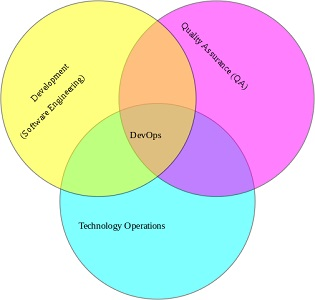
\includegraphics[scale=0.75]{imagenes/Introduccion/Conceptos_Basicos/devops.jpg}
				\caption[¿Qué es DevOps?]{¿Qué es DevOps? \cite{WhatIsDe1:online}}
				\label{termino_devops}
			\end{figure}
		\end{text}
	
	\clearpage 
	
	\subsection{Integración Continua (CI)}
		\begin{text}
			La Integración Continua o CI para abreviar, es uno de los pilares de la filosofía DevOps. La integración continua se basa en hacer integraciones automáticas de un proyecto lo más a menudo posible para poder detectar fallos rápidamente. Consta de dos partes: compilación y ejecución de test de un proyecto.
			
			
			\begin{figure}[!hbt]
				\centering
				\includegraphics[scale=0.45]{imagenes/Introduccion/Conceptos_Basicos/ci.png}
				\caption[Integración Continua]{Integración Continua \cite{Alcanzan90:online} }
				\label{integracion_continua} 
			\end{figure}
		\end{text}
	\subsection{Despliegue continuo (CD)}
		\begin{text}
			El despliegue continuo o CD por sus siglas en inglés 'continous delivery' complementa a la integración continua desplegando el proyecto software en los servidores, una vez ha pasado el proceso de la integración continua. Gracias a 'continous delivery' podemos garantizar entregas rápidas y seguras de software.
			
			\begin{figure}[!hbt]
				\centering
				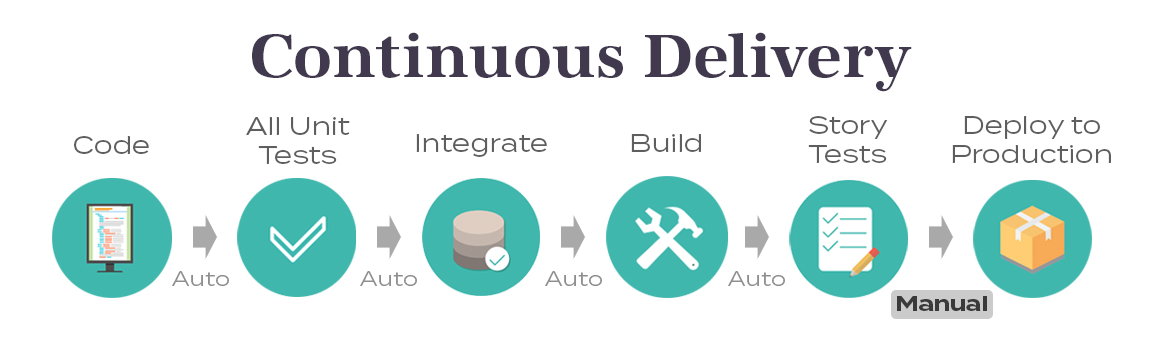
\includegraphics[scale=0.35]{imagenes/Introduccion/Conceptos_Basicos/CD.png}
				\caption[Despliegue Continuo]{Despliegue Continuo \cite{continuo84:online}}
				\label{despligue_continuo} 
			\end{figure}
		\end{text}
	\subsection{Infraestructura como Código (IaaC)}
		\begin{text}
			La infraestructura como código pretende tratar los servidores y toda la infraestructura alrededor de una organización como un software de programación. De este modo, la infraestructura está escrita en ficheros de configuración y es fácilmente replicable y testeable. Este concepto al igual que los dos anteriores está íntimamente ligado con el término DevOps, ya que es uno de los primeros pasos a adoptar. IaaC pretende difuminar la línea entre el código que ejecutan las aplicaciones y el código que configura la infraestructura. Acerca a los desarrolladores al equipo de operaciones o administradores de sistemas. \\
			De esta manera no únicamente se testea el software antes de ser lanzado, si no también la infraestructura. A continuación se muestra como sería el cauce de trabajo siguiendo los principios de IaaC.
			
			\begin{figure}[!hbt]
				\centering
				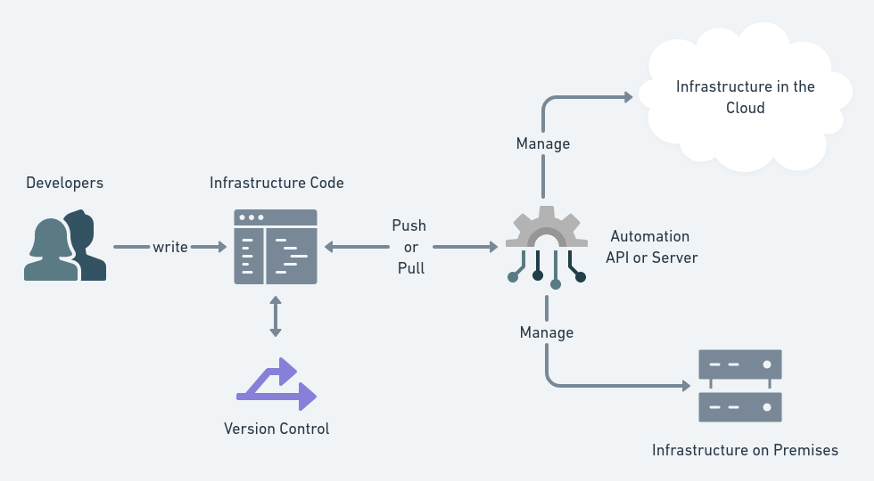
\includegraphics[scale=0.75]{imagenes/Introduccion/Conceptos_Basicos/IaaC.png}
				\caption[Infraestructura como Código]{Infraestructura como Código \cite{WhatIsIaaC:online}}
				\label{infraestructura_como_codigo} 
			\end{figure}
		\end{text}
	
\section{Solución propuesta}
\begin{text}
	Este proyecto se ha creado para cumplir con los objetivos descritos en la sección \nameref{objetivos_primarios}. A continuación se define a grandes rasgos la solución propuesta que se irá justificando y ampliando a lo largo del documento. \\
	\begin{itemize}
		\item \textbf{Objetivo 1: Asegurar unos tiempos bajos en la creación de infraestructura para proveer servicios}. \\ Aplicando la filosofía DevOps a la infraestructura. Se tratará la infraestructura como si fuese un proyecto software, es decir, la infraestructura será codificada bajo ficheros de configuración y estos estarán alojados en algún sistema de control de versiones.
		\item \textbf{Objetivo 1.1: Infraestructura segura frente a ataques}. \\ Para garantizar la seguridad de la infraestructura, se desplegarán firewalls redundantes. Estos firewalls serán tratados como servicios y entran dentro de las especificaciones del objetivo 3.
		\item \textbf{Objetivo 2: Replicar la infraestructura asegurando bajos tiempos de creación.} \\
		Si se consigue objetivo 1, es decir, tener la infraestructura codificada en ficheros de configuración con alguna herramienta de automatización, esta será fácilmente replicable. Si se cumple el objetivo 1, se cumplirá el objetivo 2.
		\item \textbf{Objetivo 3: Crear y desplegar servicios necesarios para una empresa de aplicaciones web asegurando bajos tiempos de creación.} \\
		Una vez cumplidos objetivos 1 y 2, y con una infraestructura base desplegada, será necesario desplegar los servicios que una empresa, dedicada al desarrollo de aplicaciones, web requiere. Servicios como servidores web, servicios de orquestación de contenedores, gestor de paso de mensajes... Para garantizar que estos servicios se pueden crear y desplegar en tiempos eficientes, será necesario utilizar herramientas de automatización, de manera que, mediante ficheros de configuración lanzados en la infraestructura, logramos el despliegue de todos los servicios necesarios.
		\item \textbf{Objetivo 4: Crear cauces rápidos y seguros para la creación de nuevo software.} \\
		Para cumplir con este objetivo se va a instalar un servicio en la infraestructura que permita la creación de dichos cauces. Se aplicarán técnicas para garantizar los despliegues automáticos y la creación de entornos de pruebas para probar las aplicaciones. La seguridad está garantizada ya que todo sucede en un entorno seguro gracias al subobjetivo 1.1, y en una red LAN a la cual únicamente tienen acceso los administradores.
	\end{itemize}
\end{text}

